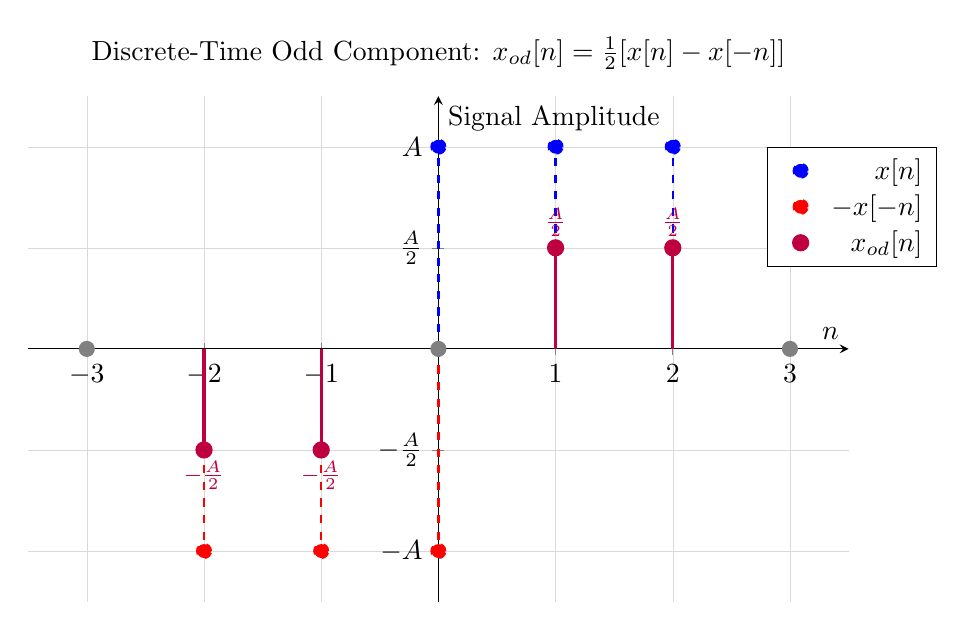
\begin{tikzpicture}
	% Define styles for the different stem plots
	\pgfplotsset{
		impulse/.style={ ycomb, thick, mark=*, mark size=2.5pt },
		original/.style={ impulse, blue, dashed },
		reversed_neg/.style={ impulse, red, dashed },
		odd/.style={ impulse, purple, very thick },
	}
	
	\begin{axis}[
		% Set the overall style
		width=12cm,
		height=8cm,
		% Title with the definition of the odd component
		title={Discrete-Time Odd Component: $x_{od}[n] = \frac{1}{2}[x[n] - x[-n]]$},
		% Axis labels
		xlabel={$n$},
		ylabel={Signal Amplitude},
		% Position axes at the origin
		axis lines=middle,
		% Set axis limits
		xmin=-3.5, xmax=3.5,
		ymin=-2.5, ymax=2.5,
		% Set ticks at key points
		xtick={-3, -2, -1, 0, 1, 2, 3},
		ytick={-2, -1, 1, 2},
		yticklabels={$-A$, $-\frac{A}{2}$, $\frac{A}{2}$, $A$},
		% Add a grid
		grid=major,
		grid style={line width=.1pt, draw=gray!30},
		% Position the legend
		legend style={
	at={(0.9, 0.9)}, % 3% from left, 97% from bottom
	anchor=north west,   % Anchor the top-left corner of the legend
	legend cell align={right}
},
		]
		
		% 1. Plot the original signal (dashed blue)
		\addplot[original] coordinates {(0,2) (1,2) (2,2)};
		\addlegendentry{$x[n]$};
		
		% 2. Plot the negative time-reversed signal (dashed red)
		\addplot[reversed_neg] coordinates {(-2,-2) (-1,-2) (0,-2)};
		\addlegendentry{$-x[-n]$};
		
		% 3. Plot the resulting odd component (solid purple)
		% Plot the positive values with labels above
		\addplot[
		odd,
		nodes near coords={$\frac{A}{2}$},
		every node near coord/.style={anchor=south, font=\footnotesize},
		] coordinates {(1,1) (2,1)};
		\addlegendentry{$x_{od}[n]$};
		
		% Plot the negative values with labels below
		\addplot[
		odd,
		nodes near coords=$-\frac{A}{2}$,
		every node near coord/.style={anchor=north, font=\footnotesize},
		] coordinates {(-2,-1) (-1,-1)};
		
		% Plot the zero-value points for context
		\addplot[impulse, gray] coordinates {(-3,0) (0,0) (3,0)};
		
	\end{axis}
\end{tikzpicture}